% =============================================================================
%  fig_research_loop.tex  —  "One generation of the framework"
%  Figure for Section~\ref{sec:fw_loop}.
%
%  HOW TO USE
%  ----------
%  (A) Standalone preview / export a cropped PDF:
%        pdflatex fig_research_loop.tex   ->  fig_research_loop.pdf
%      then 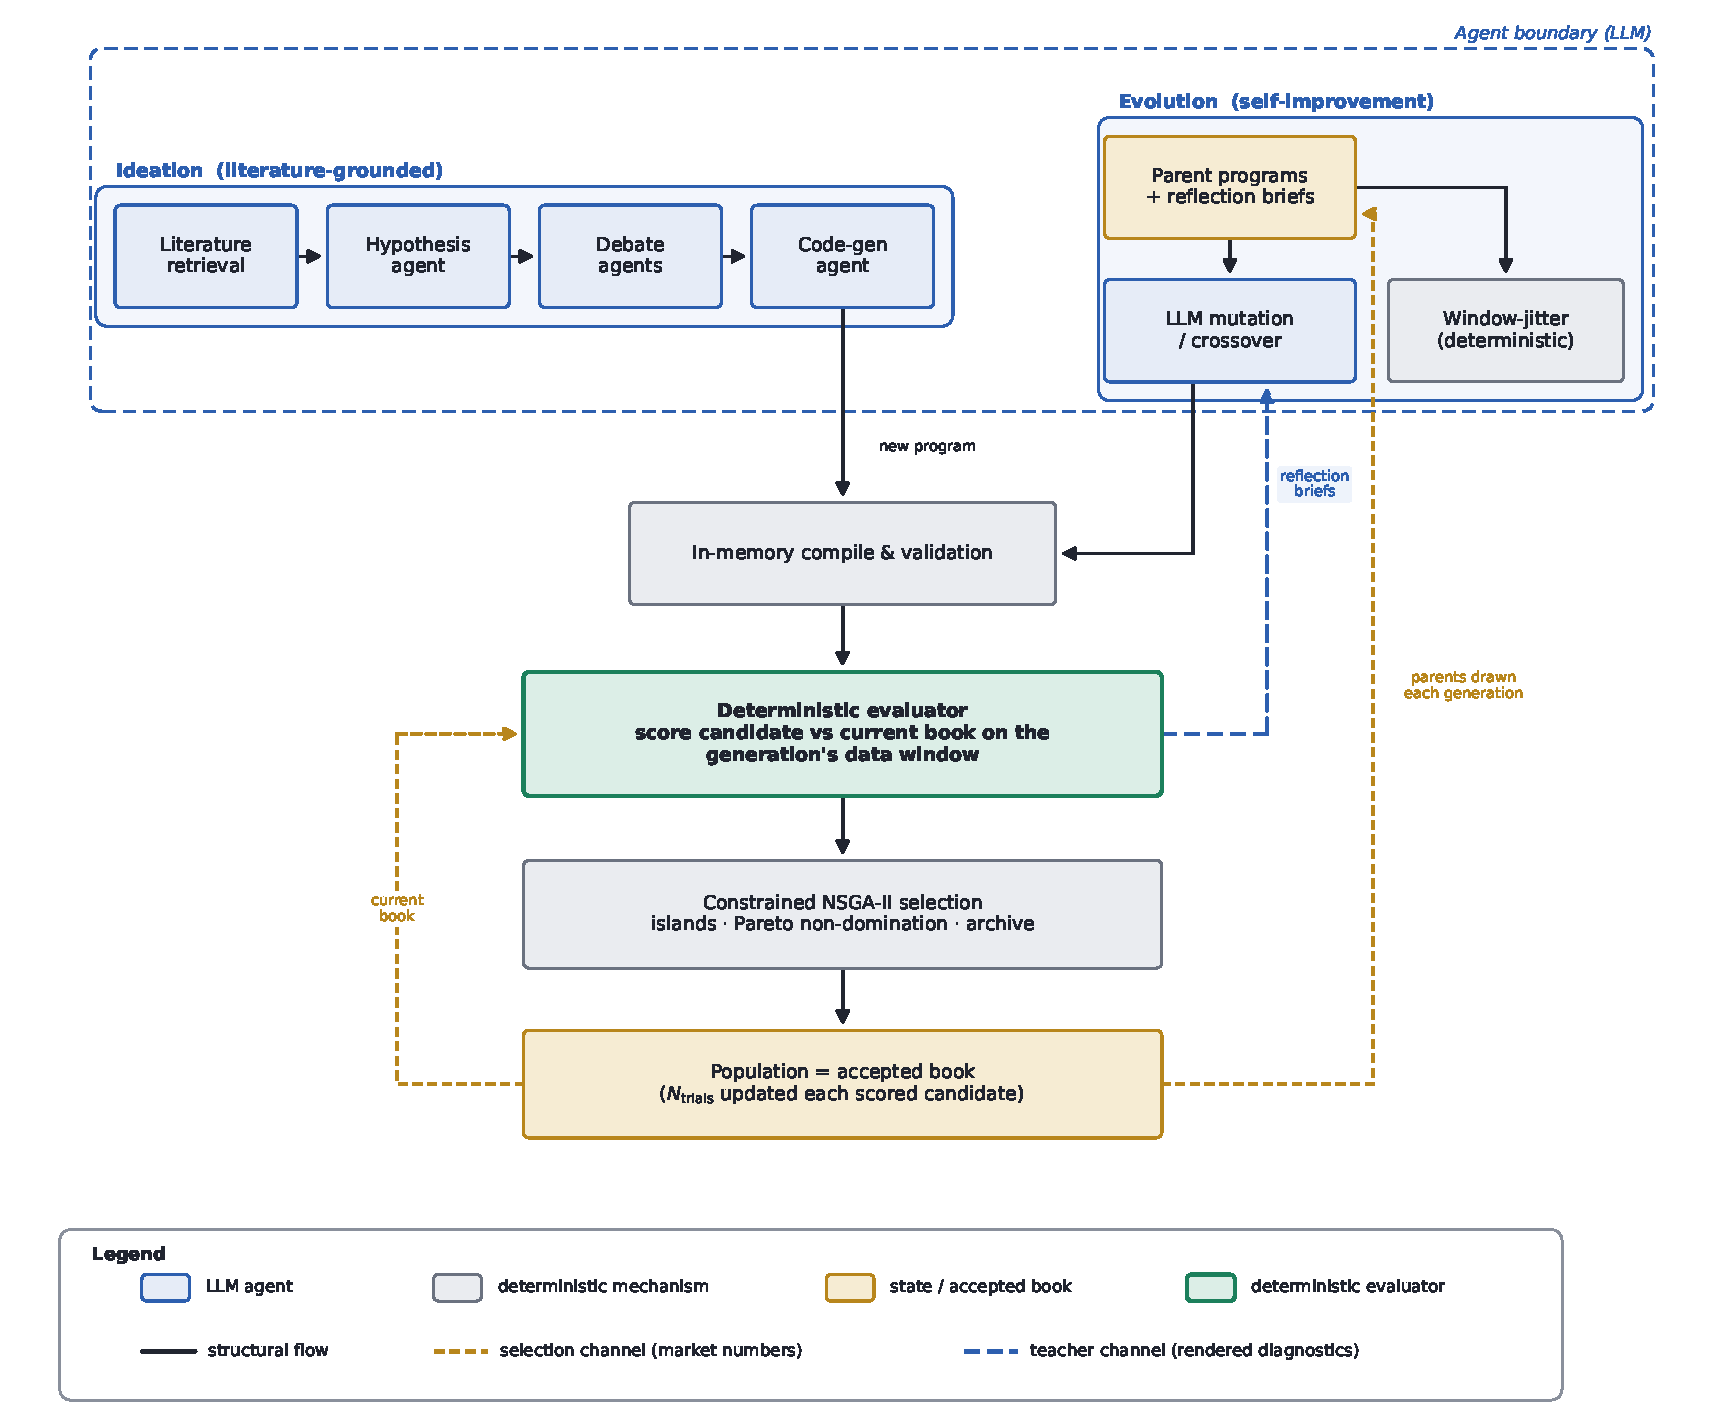
\includegraphics{fig_research_loop} in the thesis.
%
%  (B) Inline in the thesis: comment out the \documentclass..\begin{document}
%      and ..\end{document} lines (marked <<STANDALONE>>), move the four
%      \definecolor lines and \usetikzlibrary line into your preamble, and
%      \input this file inside a figure environment.
% =============================================================================

% <<STANDALONE>> ---------------------------------------------------------------
\documentclass[border=6pt]{standalone}
\usepackage{amsmath}
\usepackage{tikz}
% -----------------------------------------------------------------------------

\usetikzlibrary{arrows.meta,positioning,fit,backgrounds,calc}

% --- Palette (muted, print-safe; consistent with the framework chapter) ------
\definecolor{Ink}{RGB}{33,37,48}        % near-black text / structural flow
\definecolor{AgentBlue}{RGB}{45,95,175}  % LLM agents + teacher channel
\definecolor{DataGold}{RGB}{184,134,28}  % state / data / market-number channel
\definecolor{EvalGreen}{RGB}{28,128,92}  % deterministic evaluator
\definecolor{SoftGrey}{RGB}{234,236,240} % deterministic-mechanism fill

\begin{document}  % <<STANDALONE>>

\begin{tikzpicture}[
  x=1cm, y=1cm,
  font=\sffamily\scriptsize,
  >=Latex,
  % --- edge (channel) styles --------------------------------------------------
  flow/.style     ={-{Latex[length=2.2mm,width=1.5mm]}, draw=Ink,
                    line width=0.7pt, rounded corners=2pt},
  teacher/.style  ={-{Latex[length=2.2mm,width=1.5mm]}, draw=AgentBlue,
                    line width=0.8pt, dashed, rounded corners=2pt},
  dataflow/.style ={-{Latex[length=2.2mm,width=1.5mm]}, draw=DataGold,
                    line width=0.8pt, dash pattern=on 2.6pt off 1.6pt,
                    rounded corners=2pt},
  % --- node (role) styles -----------------------------------------------------
  base/.style ={draw=Ink!72, line width=0.55pt, rounded corners=2.4pt,
                minimum height=0.9cm, align=center, inner sep=4pt},
  agent/.style        ={base, fill=AgentBlue!10, draw=AgentBlue!85},
  deterministic/.style={base, fill=SoftGrey, draw=Ink!55},
  state/.style        ={base, fill=DataGold!12, draw=DataGold!85},
  evaluator/.style    ={base, fill=EvalGreen!11, draw=EvalGreen!90,
                        line width=0.9pt},
  group/.style ={rounded corners=3pt, line width=0.6pt, inner sep=7pt},
  glab/.style  ={font=\sffamily\bfseries\scriptsize, text=Ink},
  elab/.style  ={font=\sffamily\tiny, text=Ink!85, fill=white,
                inner sep=1.4pt, align=center},
]

% ===========================================================================
%  ENTRY PATH I — literature-grounded ideation  (generation 0 / one-shot arm)
% ===========================================================================
\node[agent, text width=1.5cm] (retrieval)  at (0.95,8.35) {Literature\\retrieval};
\node[agent, text width=1.5cm] (hypothesis) at (2.85,8.35) {Hypothesis\\agent};
\node[agent, text width=1.5cm] (debate)     at (4.75,8.35) {Debate\\agents};
\node[agent, text width=1.5cm] (codegen)    at (6.65,8.35) {Code-gen\\agent};

\draw[flow] (retrieval)  -- (hypothesis);
\draw[flow] (hypothesis) -- (debate);
\draw[flow] (debate)     -- (codegen);

% ===========================================================================
%  ENTRY PATH II — evolution of existing factors  (generations >= 1)
% ===========================================================================
\node[state, text width=2.05cm] (parents) at (9.55,8.95)
  {Parent programs\\ + reflection briefs};
\node[agent, text width=2.05cm] (variate) at (9.55,7.75)
  {LLM mutation\\ / crossover};
\node[deterministic, text width=2.05cm] (jitter) at (12.05,7.75)
  {Window-jitter\\(deterministic)};

\draw[flow] (parents) -- (variate);
\draw[flow] (parents.east) -- ++(0.55,0) |- (jitter.east);

% ===========================================================================
%  DETERMINISTIC CORE — compile -> evaluate -> select -> book  (the spine)
% ===========================================================================
\node[deterministic, text width=3.9cm] (compile) at (6.5,5.6)
  {In-memory compile \& validation};
\node[evaluator, text width=5.6cm] (evaluator) at (6.5,4.0)
  {\textbf{Deterministic evaluator}\\[1pt]
   score candidate against current book\\ on the generation's data window};
\node[deterministic, text width=5.6cm] (selection) at (6.5,2.4)
  {Constrained NSGA-II selection\\ islands $\cdot$ Pareto non-domination $\cdot$ archive};
\node[state, text width=5.6cm] (book) at (6.5,0.75)
  {Population $=$ accepted book\\ ($N_{\mathrm{trials}}$ updated each scored candidate)};

\draw[flow] (compile)   -- node[elab,pos=0.5]{new program} (evaluator);
\draw[flow] (evaluator) -- (selection);
\draw[flow] (selection) -- (book);

% --- both entry paths feed the compiler ------------------------------------
\draw[flow] (codegen.south) -- ++(0,-0.55) -| (compile.north);
\draw[flow] (variate.south) -- ++(0,-0.35) |- (compile.east);
\draw[flow] (jitter.south)  -- ++(0,-0.35) |- (compile.east);

% ===========================================================================
%  FEEDBACK CHANNELS
% ===========================================================================
% (1) selection channel: the book is the parent pool each generation (numbers)
\draw[dataflow] (book.east) -- ++(3.05,0)
      node[elab,pos=0.55]{parents drawn\\each generation}
      |- (parents.east);

% (2) selection channel: candidate is scored *against* the current book
\draw[dataflow] (book.west) -- ++(-0.85,0)
      node[elab,pos=0.5]{current\\book} |- (evaluator.west);

% (3) teacher channel: rendered diagnostics -> proposing (evolution) agents
\draw[teacher] (evaluator.east) -- ++(0.95,0)
      node[elab,pos=0.5,fill=AgentBlue!5]{reflection\\briefs}
      |- (variate.west);

% ===========================================================================
%  AGENT BOUNDARY + GROUP FRAMES (drawn behind the nodes)
% ===========================================================================
\begin{scope}[on background layer]
  % ideation group
  \node[group, draw=AgentBlue!55, fill=AgentBlue!4,
        fit=(retrieval)(codegen)] (ideabox) {};
  % evolution group
  \node[group, draw=AgentBlue!55, fill=AgentBlue!4,
        fit=(parents)(variate)(jitter)] (evobox) {};
  % agent boundary encloses the two proposer groups only (NOT the evaluator)
  \node[group, draw=AgentBlue!70, dashed, line width=0.8pt,
        fit=(ideabox)(evobox), inner sep=11pt] (agentbound) {};
\end{scope}

\node[glab, anchor=south west, text=AgentBlue!85]
  at ([yshift=1.5pt]ideabox.north west) {Ideation \small(literature-grounded)};
\node[glab, anchor=south west, text=AgentBlue!85]
  at ([yshift=1.5pt]evobox.north west) {Evolution \small(self-improvement)};
\node[glab, anchor=north east, text=AgentBlue!70]
  at ([xshift=-2pt,yshift=-2pt]agentbound.north east) {Agent boundary (LLM)};

% ===========================================================================
%  LEGEND
% ===========================================================================
\begin{scope}[shift={(0.0,-0.75)}]
  \node[group, draw=Ink!35, fill=white, anchor=north west,
        minimum width=5.0cm, align=left] (legend) at (0.0,0.0)
    {\begin{tabular}{@{}ll@{}}
       \multicolumn{2}{@{}l}{\bfseries Legend}\\[2pt]
       \tikz{\draw[agent,fill=AgentBlue!10] (0,0) rectangle (0.42,0.24);}
         & LLM agent (proposes / criticises)\\
       \tikz{\draw[deterministic] (0,0) rectangle (0.42,0.24);}
         & deterministic mechanism\\
       \tikz{\draw[state] (0,0) rectangle (0.42,0.24);}
         & state / accepted book\\
       \tikz{\draw[evaluator] (0,0) rectangle (0.42,0.24);}
         & deterministic evaluator\\[2pt]
       \tikz{\draw[flow] (0,0.12)--(0.5,0.12);}
         & structural flow\\
       \tikz{\draw[dataflow] (0,0.12)--(0.5,0.12);}
         & selection channel (market numbers)\\
       \tikz{\draw[teacher] (0,0.12)--(0.5,0.12);}
         & teacher channel (rendered diagnostics)\\
     \end{tabular}};
\end{scope}

\end{tikzpicture}

\end{document}  % <<STANDALONE>>
